%% LaTeX Beamer: Session 2 - Regresión Lineal Simple
%% Econometrics Leveling Course - PhD in Social Complexity Sciences
%% CICS-UDD | 2026

\documentclass[aspectratio=169,11pt]{beamer}
\usepackage[utf8]{inputenc}
\usepackage[T1]{fontenc}
\usepackage[english]{babel}
\usetheme{Madrid}
\usecolortheme{whale}
\definecolor{uddblue}{HTML}{1F4E79}
\definecolor{uddlight}{HTML}{2E86C1}
\setbeamercolor{structure}{fg=uddblue}
\setbeamercolor{frametitle}{bg=uddblue,fg=white}
\setbeamercolor{title}{bg=uddblue,fg=white}
\setbeamercolor{block title}{bg=uddblue,fg=white}
\setbeamercolor{block body}{bg=uddblue!10}
\setbeamercolor{item}{fg=uddblue}
\usepackage{amsmath,amssymb}
\usepackage{graphicx}
\usepackage{booktabs}
\usepackage{listings}
\usepackage{tikz}
\usetikzlibrary{shapes,arrows,positioning,calc}
\lstset{language=R,basicstyle=\ttfamily\scriptsize,keywordstyle=\color{uddblue}\bfseries,commentstyle=\color{gray},stringstyle=\color{uddlight},backgroundcolor=\color{uddblue!5},frame=single,rulecolor=\color{uddblue!30},breaklines=true,showstringspaces=false}
\graphicspath{{figuras/}}
\titlegraphic{
\includegraphics[height=1.2cm]{logo_gobierno.png}}
\institute[CICS — UDD]{Doctorado en Ciencias de la Complejidad Social — CICS, UDD}
\newcommand{\highlight}[1]{\textcolor{uddlight}{\bfseries #1}}
% Title, Author, Institute
\title{Regresión Lineal Simple}
\subtitle{Sesión 2: Modelos Económetricos Fundamentales}
\author[A. Agüero]{Amaru Agüero}
\date{24 de marzo de 2026}

%% ============================================================================
\begin{document}

%% SLIDE 1: Title
\begin{frame}[plain]
\titlepage
\end{frame}

%% SLIDE 2: Agenda
\begin{frame}
\frametitle{Agenda}
\setlength{\itemsep}{6pt}
\begin{itemize}
    \item Correlación vs.\ causalidad: conceptos fundamentales
    \item Modelo de regresión lineal simple: formulación
    \item Estimación por Mínimos Cuadrados Ordinarios (MCO/OLS)
    \item Interpretación de coeficientes
    \item Bondad de ajuste: $R^2$ y $R^2$ ajustado
    \item Errores estándar e inferencia estadística
    \item Supuestos del modelo clásico (Gauss-Markov)
    \item Implementación práctica en R
    \item Ejercicio práctico y conclusiones
\end{itemize}
\end{frame}

%% SLIDE 3: Correlación vs. Causalidad (1/2)
\begin{frame}
\frametitle{Correlación vs.\ Causalidad}
\framesubtitle{¿Qué es la correlación?}

\small
\setlength{\itemsep}{2pt}
\begin{itemize}
    \item \textbf{Correlación}: mide la asociación lineal entre dos variables
    \item Rango: $-1 \leq \rho \leq 1$
    \item \textbf{Coeficiente de Pearson}:
    $$\rho = \frac{\text{Cov}(X, Y)}{\sigma_X \sigma_Y}$$
    \item Información: fuerza y dirección de la relación
    \item \textbf{Límite}: no implica relación causa-efecto
\end{itemize}

\vspace{0.3cm}
\begin{alertblock}{Punto Clave}
    \vspace{-0.2cm}
    Correlación alta no implica causalidad: confounding, reverse causality, relaciones espurias
    \vspace{-0.15cm}
\end{alertblock}
\end{frame}

%% SLIDE 4: Correlación vs. Causalidad (2/2)
\begin{frame}
\frametitle{Correlación vs.\ Causalidad}
\framesubtitle{De la correlación a la causalidad}

\small
\setlength{\itemsep}{3pt}
\begin{itemize}
    \item \textbf{Regresión}: permite modelar la relación \textit{condicional}
    \item Bajo ciertos \textbf{supuestos}, podemos interpretar coeficientes causalmente
    \item Supuesto crítico: \textbf{exogeneidad} de los regresores
    \item Si $E[\varepsilon | X] = 0$, entonces $\beta_1$ mide el efecto causal de $X$ en $Y$
\end{itemize}

\vspace{0.6cm}
\begin{exampleblock}{Ejemplo}
    \footnotesize
    ¿Correlación entre educación y salario implica causalidad?
    \begin{itemize}
        \item Correlación: positiva y fuerte
        \item Causalidad: bajo supuestos (p.ej., habilidad no omitida)
        \item Regresión: estima el efecto ceteris paribus
    \end{itemize}
\end{exampleblock}
\end{frame}

%% SLIDE 5: Modelo de Regresión Lineal Simple (1/2)
\begin{frame}
\frametitle{Modelo de Regresión Lineal Simple}
\framesubtitle{Formulación general}

\begin{block}{Modelo poblacional}
$$Y = \beta_0 + \beta_1 X + \varepsilon$$
\end{block}

\small
\vspace{0.3cm}
\textbf{Notación y componentes:}
\setlength{\itemsep}{3pt}
\begin{itemize}
    \item $Y$: variable dependiente (endógena)
    \item $X$: variable independiente (exógena)
    \item $\beta_0$: intercepto (parámetro poblacional)
    \item $\beta_1$: pendiente (parámetro de interés)
    \item $\varepsilon$: término de error (inobservable)
\end{itemize}

\vspace{0.2cm}
\textbf{Interpretación ceteris paribus:}
$$\beta_1 = \frac{\partial E[Y|X]}{\partial X}$$
\end{frame}

%% SLIDE 6: Modelo de Regresión Lineal Simple (2/2)
\begin{frame}
\frametitle{Modelo de Regresión Lineal Simple}
\framesubtitle{Visualización}

\begin{center}
    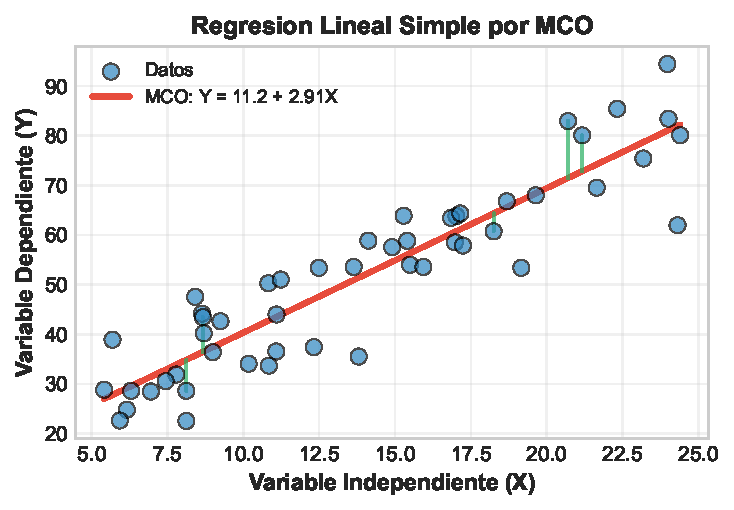
\includegraphics[height=0.55\textheight,keepaspectratio]{scatter_regresion.pdf}
\end{center}

\small
\vspace{0.2cm}
Línea roja: $\hat{Y} = \hat{\beta}_0 + \hat{\beta}_1 X$ (recta estimada)

Puntos: pares observados $(X_i, Y_i)$ con su error $\hat{\varepsilon}_i = Y_i - \hat{Y}_i$
\end{frame}

%% SLIDE 7: Estimación MCO (1/2)
\begin{frame}
\frametitle{Estimación por Mínimos Cuadrados Ordinarios}
\framesubtitle{Principio y derivación intuitiva}

\small
\textbf{Objetivo}: minimizar la suma de errores al cuadrado (SSE)
$$SSE = \sum_{i=1}^{n} \varepsilon_i^2 = \sum_{i=1}^{n} (Y_i - \beta_0 - \beta_1 X_i)^2$$

\vspace{0.3cm}
\textbf{Condiciones de primer orden} (igualando derivadas a cero):
$$\frac{\partial SSE}{\partial \beta_0} = -2 \sum_i (Y_i - \beta_0 - \beta_1 X_i) = 0$$
$$\frac{\partial SSE}{\partial \beta_1} = -2 \sum_i X_i(Y_i - \beta_0 - \beta_1 X_i) = 0$$

\vspace{0.3cm}
\textbf{Resultado}: sistema de ecuaciones normales que se resuelve para $\hat{\beta}_0$ y $\hat{\beta}_1$.
\end{frame}

%% SLIDE 8: Estimación MCO (2/2)
\begin{frame}
\frametitle{Estimación por Mínimos Cuadrados Ordinarios}
\framesubtitle{Fórmulas de los estimadores}

\small
\begin{alertblock}{Estimadores MCO}
    $$\hat{\beta}_1 = \frac{\sum_{i=1}^{n}(X_i - \bar{X})(Y_i - \bar{Y})}{\sum_{i=1}^{n}(X_i - \bar{X})^2} = \frac{\text{Cov}(X,Y)}{\text{Var}(X)}$$

    $$\hat{\beta}_0 = \bar{Y} - \hat{\beta}_1 \bar{X}$$
\end{alertblock}

\vspace{0.4cm}
\textbf{Propiedades (bajo supuestos):}
\setlength{\itemsep}{2pt}
\begin{itemize}
    \item Insesgados: $E[\hat{\beta}_j] = \beta_j$
    \item Consistentes: $\hat{\beta}_j \xrightarrow{p} \beta_j$
    \item Eficientes: varianza mínima entre estimadores lineales insesgados (BLUE)
\end{itemize}
\end{frame}

%% SLIDE 9: Interpretación de Coeficientes (1/2)
\begin{frame}
\frametitle{Interpretación de Coeficientes}
\framesubtitle{Significado económico}

\small
\textbf{Pendiente $\hat{\beta}_1$:}
\setlength{\itemsep}{2pt}
\begin{itemize}
    \item Cambio en $Y$ cuando $X$ aumenta en una unidad
    \item Efecto marginal ceteris paribus
    \item Unidades: mismo ratio que $\frac{[Y]}{[X]}$
\end{itemize}

\vspace{0.4cm}
\textbf{Ejemplo:} Si $Y$ = salario (USD/año) y $X$ = educación (años)
\begin{itemize}
    \item $\hat{\beta}_1 = 2000$ significa: 1 año adicional de educación $\Rightarrow$ +USD 2000 de salario
\end{itemize}

\vspace{0.4cm}
\textbf{Intercepto $\hat{\beta}_0$:}
\begin{itemize}
    \item Valor predicho de $Y$ cuando $X = 0$
    \item Interpretación económica no siempre directa
    \item Referencia para la recta de regresión
\end{itemize}
\end{frame}

%% SLIDE 10: Interpretación de Coeficientes (2/2)
\begin{frame}
\frametitle{Interpretación de Coeficientes}
\framesubtitle{Transformaciones logarítmicas}

\small
\begin{tabular}{lll}
    \toprule
    \textbf{Modelo} & \textbf{Forma} & \textbf{Interpretación de $\hat{\beta}_1$} \\
    \midrule
    Lineal & $Y = \beta_0 + \beta_1 X + \varepsilon$ & Cambio absoluto en $Y$ \\
    Log-Log & $\ln Y = \beta_0 + \beta_1 \ln X + \varepsilon$ & Elasticidad (\% cambio) \\
    Log-Lin & $\ln Y = \beta_0 + \beta_1 X + \varepsilon$ & Cambio \% en $Y$ \\
    Lin-Log & $Y = \beta_0 + \beta_1 \ln X + \varepsilon$ & Cambio en $Y$ por \% cambio en $X$ \\
    \bottomrule
\end{tabular}

\vspace{0.6cm}
\small
\textbf{Ejemplo Log-Log:} Si $\hat{\beta}_1 = 0.5$, entonces un aumento de 1\% en $X$
implica un aumento de 0.5\% en $Y$ (elasticidad de demanda, etc.).
\end{frame}

%% SLIDE 11: Bondad de Ajuste (1/2)
\begin{frame}
\frametitle{Bondad de Ajuste: $R^2$ y $R^2$ Ajustado}
\framesubtitle{Medidas de explicación de variabilidad}

\small
\textbf{Descomposición de variabilidad:}
\begin{itemize}
    \item $SST = SSE + SSR$ \quad (suma total = suma explicada + suma residual)
    \item $\sum(Y_i - \bar{Y})^2 = \sum(Y_i - \hat{Y}_i)^2 + \sum(\hat{Y}_i - \bar{Y})^2$
\end{itemize}

\vspace{0.3cm}
\begin{block}{Coeficiente de determinación}
    $$R^2 = 1 - \frac{SSE}{SST} = \frac{SSR}{SST}$$
    Proporción de varianza en $Y$ explicada por $X$ (rango: $[0,1]$)
\end{block}

\vspace{0.3cm}
\textbf{$R^2$ ajustado:} penaliza por número de regresores
$$\bar{R}^2 = 1 - \frac{SSE/(n-k)}{SST/(n-1)}$$
donde $k$ = número de parámetros, $n$ = número de observaciones.
\end{frame}

%% SLIDE 12: Bondad de Ajuste (2/2)
\begin{frame}
\frametitle{Bondad de Ajuste: Visualización}

\begin{center}
    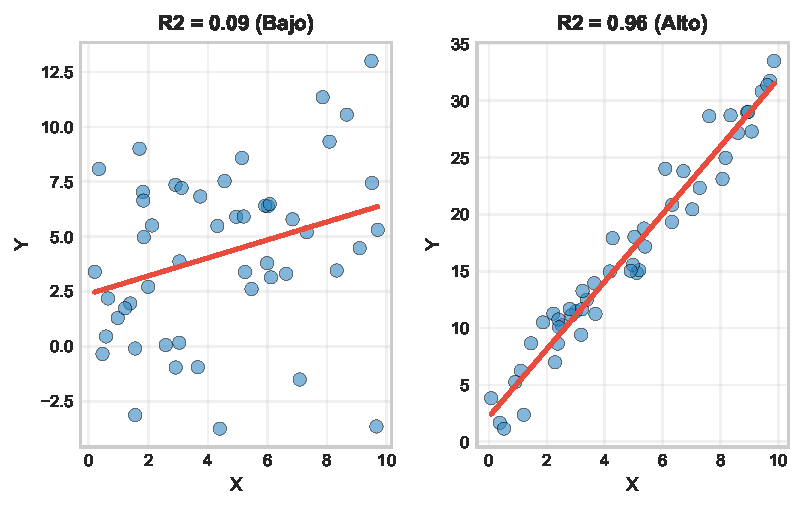
\includegraphics[height=0.55\textheight,keepaspectratio]{r_cuadrado.pdf}
\end{center}

\small
Izquierda: bajo $R^2$ (residuos grandes) | Derecha: alto $R^2$ (residuos pequeños)
\end{frame}

%% SLIDE 13: Errores Estándar e Inferencia (1/2)
\begin{frame}
\frametitle{Errores Estándar e Inferencia Estadística}
\framesubtitle{Varianza de los estimadores}

\small
\textbf{Varianza residual:} $\hat{\sigma}^2 = \frac{SSE}{n-2}$, \quad $SE(\hat{\beta}_1) = \frac{\hat{\sigma}}{\sqrt{\sum_i(X_i - \bar{X})^2}}$

\vspace{0.1cm}
\begin{alertblock}{Prueba $t$ de significancia}
    $t = \frac{\hat{\beta}_1}{SE(\hat{\beta}_1)} \sim t_{n-2}$ \quad | \quad $H_0: \beta_1 = 0$ vs $H_1: \beta_1 \neq 0$
\end{alertblock}

\vspace{0.1cm}
\textbf{IC 95\%:} $\hat{\beta}_1 \pm t_{0.025, n-2} \cdot SE(\hat{\beta}_1)$
\end{frame}

%% SLIDE 14: Errores Estándar e Inferencia (2/2)
\begin{frame}
\frametitle{Errores Estándar e Inferencia Estadística}
\framesubtitle{Interpretación de resultados}

\small
\textbf{Salida típica de software (ej. R):}

\begin{table}
    \centering
    \footnotesize
    \begin{tabular}{lrrrr}
        \toprule
        & Coef. & SE & t-stat & p-valor \\
        \midrule
        (Intercept) & $\hat{\beta}_0$ & $SE(\hat{\beta}_0)$ & $t_0$ & $p_0$ \\
        $X$ & $\hat{\beta}_1$ & $SE(\hat{\beta}_1)$ & $t_1$ & $p_1$ \\
        \bottomrule
    \end{tabular}
\end{table}

\vspace{0.4cm}
\textbf{Regla de decisión:}
\begin{itemize}
    \item Si $p\text{-valor} < 0.05 \Rightarrow$ rechazamos $H_0$ (coeficiente significativo)
    \item Si $p\text{-valor} \geq 0.05 \Rightarrow$ no rechazamos $H_0$
\end{itemize}

\vspace{0.3cm}
\textbf{Nota:} Significancia estadística $\neq$ significancia económica/práctica
\end{frame}

%% SLIDE 15: Supuestos Gauss-Markov (1/2)
\begin{frame}
\frametitle{Supuestos del Modelo Clásico}
\framesubtitle{Condiciones para la validez de MCO}

\small
\setlength{\itemsep}{3pt}
\begin{enumerate}
    \item \textbf{Linealidad}: relación lineal en parámetros: $Y = \beta_0 + \beta_1 X + \varepsilon$

    \item \textbf{Exogeneidad}: $E[\varepsilon | X] = 0$ (errores no correlacionados con $X$)

    \item \textbf{Sin multicolinealidad exacta}: varianza de $X$ es positiva y finita

    \item \textbf{Homocedasticidad}: $\text{Var}(\varepsilon | X) = \sigma^2$ (varianza constante)

    \item \textbf{Sin autocorrelación}: $\text{Cov}(\varepsilon_i, \varepsilon_j | X) = 0$ para $i \neq j$

    \item \textbf{Normalidad} (para inferencia): $\varepsilon \sim N(0, \sigma^2)$
\end{enumerate}

\vspace{0.4cm}
\small
\textbf{Teorema Gauss-Markov:} Bajo supuestos 1–5, MCO es el estimador BLUE
(mejor linealmente insesgado).
\end{frame}

%% SLIDE 16: Supuestos Gauss-Markov (2/2)
\begin{frame}
\frametitle{Diagnóstico de Supuestos}
\framesubtitle{Gráficos de residuos}

\begin{center}
    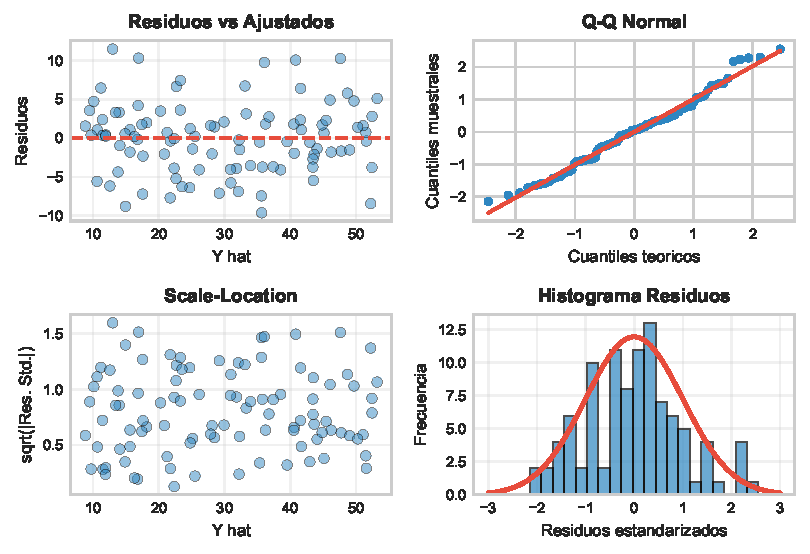
\includegraphics[height=0.55\textheight,keepaspectratio]{supuestos_ols.pdf}
\end{center}

\small
Paneles: Residuos vs. Ajustados | Q-Q plot | Scale-Location | Residuos vs. Palanca
\end{frame}

%% SLIDE 17: Implementación en R (1/2)
\begin{frame}[fragile]
\frametitle{Implementación Práctica en R}
\framesubtitle{Estimación del modelo}

\begin{lstlisting}
# Cargar datos
data(mtcars)

# Linear regression: mpg ~ wt
modelo <- lm(mpg ~ wt, data = mtcars)

# Resumen detallado
summary(modelo)
\end{lstlisting}

\small
\vspace{0.3cm}
Salida: coeficientes, errores estándar, t-estadísticos, p-valores, $R^2$, prueba F global.
\end{frame}

%% SLIDE 18: Implementación en R (2/2)
\begin{frame}[fragile]
\frametitle{Implementación Práctica en R}
\framesubtitle{Gráficos de diagnóstico}

\begin{lstlisting}
# Diagnostic plots (4 panels)
plot(modelo)

# Predictions
predichos <- predict(modelo)

# Residuos
residuos <- residuals(modelo)

# Acceso a componentes
coef(modelo)        # Coeficientes
confint(modelo)     # Intervalos de confianza
\end{lstlisting}

\small
\vspace{0.3cm}
El comando \texttt{plot()} automáticamente genera los 4 gráficos estándar de diagnóstico.
\end{frame}

%% SLIDE 19: Ejercicio Práctico
\begin{frame}
\frametitle{Ejercicio Práctico}

\small
\textbf{Datos}: Dataset \texttt{mtcars} (Motor Trend Car Road Tests)

\vspace{0.3cm}
\textbf{Pregunta}: ¿Cómo el peso del automóvil afecta el consumo de combustible?

\vspace{0.3cm}
\textbf{Tareas}:
\setlength{\itemsep}{3pt}
\begin{enumerate}
    \item Estimar el modelo: $\text{mpg} = \beta_0 + \beta_1 \text{wt} + \varepsilon$

    \item Interpretar $\hat{\beta}_1$ (¿unidades? ¿signo? ¿magnitud?)

    \item ¿Es $\hat{\beta}_1$ estadísticamente significativo al 5\%?

    \item Calcular $R^2$ e interpretar (¿qué \% de variación explica?)

    \item Realizar diagnóstico gráfico de supuestos (\texttt{plot(modelo)})

    \item ¿Se cumplen los supuestos? Comentar sobre heterocedasticidad y normalidad
\end{enumerate}
\end{frame}

%% SLIDE 20: Resumen y Próxima Sesión
\begin{frame}
\frametitle{Resumen y Próximas Sesiones}

\small
\textbf{Conceptos clave de hoy:}
\setlength{\itemsep}{2pt}
\begin{itemize}
    \item Regresión vs. correlación: causalidad requiere supuestos
    \item MCO minimiza suma de cuadrados de residuos
    \item Coeficientes se interpretan como efectos marginales ceteris paribus
    \item $R^2$ mide la proporción de varianza explicada
    \item Supuestos Gauss-Markov garantizan optimalidad de MCO
    \item Diagnóstico de supuestos es fundamental
\end{itemize}

\vspace{0.5cm}
\textbf{Próximas sesiones:}
\begin{itemize}
    \item Sesión 3: Regresión múltiple (múltiples regresores)
    \item Sesión 4: Violación de supuestos y métodos robustos
    \item Sesión 5: Variables categóricas y especificación
\end{itemize}
\end{frame}

%% ============================================================================
\end{document}
